\documentclass[tikz,border=2pt]{standalone}
\usepackage{tikz,pgfplots,pgf,calc,fp}
\usepackage{letltxmacro}
\usetikzlibrary{arrows,decorations.markings,calc}
\usepackage{ifthen}
\begin{document}
\newcommand{\q}{0}
\newcommand{\w}{2}
\newcommand{\lvar}{1}
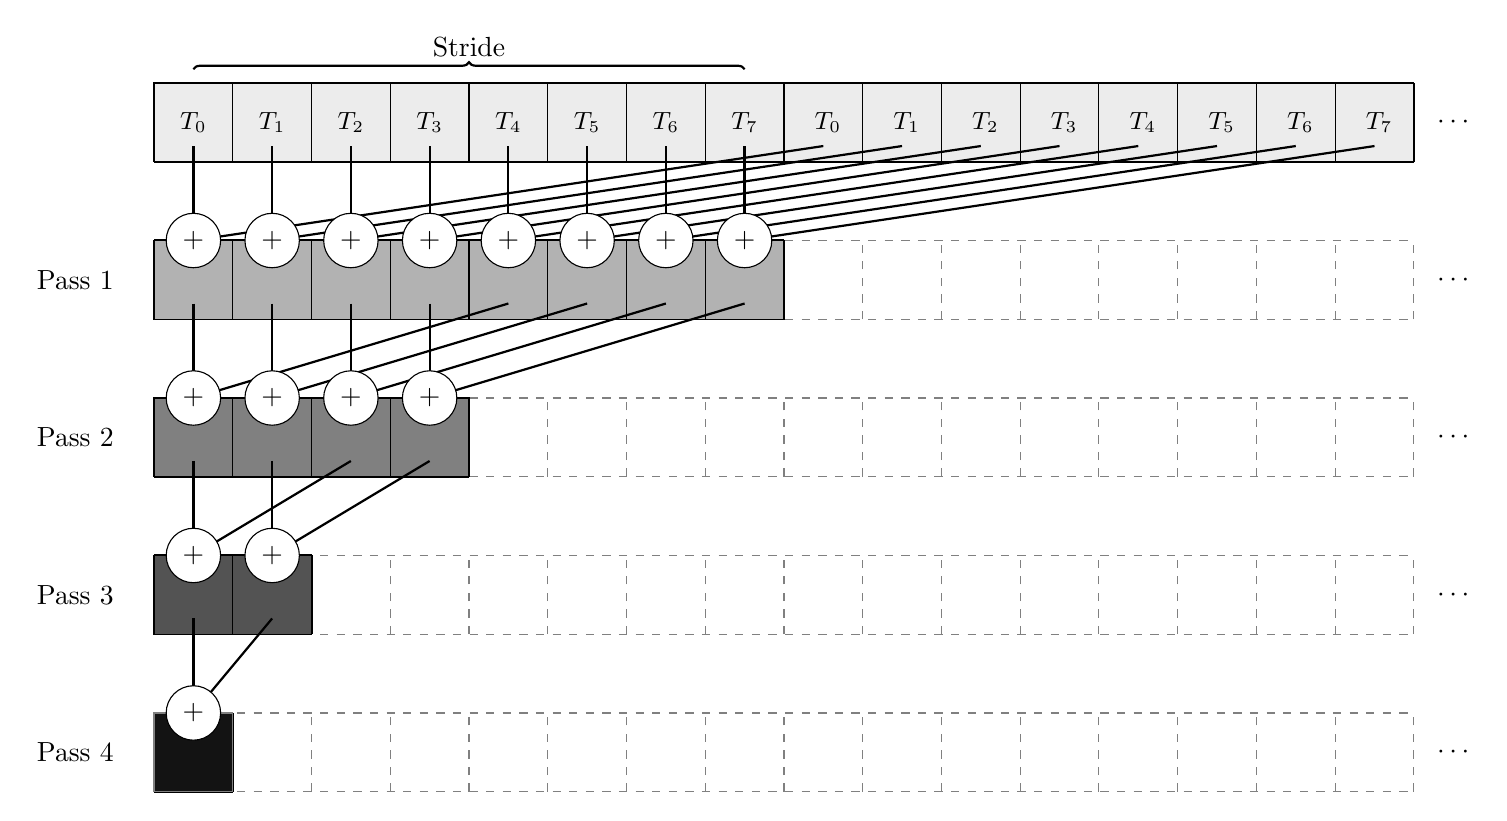
\begin{tikzpicture}[box/.style={rectangle,minimum size=1cm}]
    %\draw[step=2cm, gray, thin,dashed] (0,0) grid (8,8);
    \tikzstyle{filled} = [circle,draw,fill=white,font={}]

\draw[decoration={brace,raise=5pt},decorate,thick]
      (0.5,9) -- node[above=6pt] {Stride} (7.5,9);


\foreach \j [evaluate=\j as \b using 2^(\j/2)] in {8,6,4,2,0}{

    \draw [step=1.0, thick] (0,\j) grid (\b,\j+1);
    \ifthenelse{\not\equal{\j}{8}}{\node[] at (-1,\j+0.5) {\FPeval{\result}{clip(4-\j/2)}Pass \result};}

    \draw [step=1.0, gray, thin,dashed] (0,\j) grid (16,\j+1);
}

\foreach \i in {0,1,...,15}{
    \foreach \j in {8}{
        \node[box,draw=black,fill=white!85!gray] at (\i+0.5,\j+0.5){};

        \ifthenelse{\equal{\j}{8} \AND \i < 8}
        {
            \node[box,draw=black,fill=white!85!gray] at (\i+0.5,\j+0.5){
                \small $T_{\i}$
            };
        }{
        \node[box,draw=black,fill=white!85!gray] at (\i+0.5,\j+0.5){
            \pgfmathtruncatemacro{\jn}{mod(\i,8)}
            \small $T_{\jn}$
        };
        }


    }
}
\node at (16.5,8.5) {$\cdots$};
\node at (16.5,6.5) {$\cdots$};
\node at (16.5,4.5) {$\cdots$};
\node at (16.5,2.5) {$\cdots$};
\node at (16.5,0.5) {$\cdots$};

\foreach \i in {0,1,...,7}{
    \draw[thick,-] (\i+8.5,{8.2}) to (\i+0.5,{7. });
    \draw[thick,-] (\i+0.5,{8.2}) to (\i+0.5,{7. });
    \foreach \j in {6}{
        \node[box,draw=black,fill=white!40!gray] at (\i+0.5,\j+0.5){};
    }
    \node[filled](\i+0.5,{7 }) at (\i+0.5,{7 }) {$+$};
}


\foreach \i in {0,1,...,3}{
    \draw[thick,-] (\i+4.5,{6.2}) to (\i+0.5,{5. });
    \draw[thick,-] (\i+0.5,{6.2}) to (\i+0.5,{5. });
    \foreach \j in {4}{
        \node[box,draw=black,fill=gray] at (\i+0.5,\j+0.5){};
    }
    \node[filled](\i+0.5,{5 }) at (\i+0.5,{5 }) {$+$};
}

\foreach \i in {0,1}{
    \draw[thick,-] (\i+2.5,{4.2}) to (\i+0.5,{3. });
    \draw[thick,-] (\i+0.5,{4.2}) to (\i+0.5,{3. });
    \foreach \j in {2}{
        \node[box,draw=black,fill=gray!65!black] at (\i+0.5,\j+0.5){};
    }
    %\node[box,draw=gray,fill=gray!15!black] at (\i+0.5,+0.5){};
    \node[filled](\i+0.5,{3 }) at (\i+0.5,{3 }) {$+$};
}

\foreach \i in {0}{
    \draw[thick,-] (\i+1.5,{2.2}) to (\i+0.5,{1. });
    \draw[thick,-] (\i+0.5,{2.2}) to (\i+0.5,{1. });
    \node[box,draw=gray,fill=gray!15!black] at (\i+0.5,+0.5){};
    \node[filled](\i+0.5,{1 }) at (\i+0.5,{1 }) {$+$};
}

\end{tikzpicture}

\end{document}
